%!TEX root = ../template.tex
%%%%%%%%%%%%%%%%%%%%%%%%%%%%%%%%%%%%%%%%%%%%%%%%%%%%%%%%%%%%%%%%%%%%
%% chapter3.tex
%% NOVA thesis document file
%%
%% Chapter with a short laext tutorial and examples
%%%%%%%%%%%%%%%%%%%%%%%%%%%%%%%%%%%%%%%%%%%%%%%%%%%%%%%%%%%%%%%%%%%%
\chapter{O problema e os seus desafios}
Desenhar esta \acrfull{dsl} trás consigo os problemas comuns ao desenho de linguagens de programação, bem como desafios novos e únicos relativos ao domínio músical. Alguns desses desafios foram já bastante estudado pela míriade de linguagens de programação, tanto indústriais como académicas, que já foram desenvolvidas, pelo que não serão o foco principal deste projeto. Pelo contrário, neste projeto serão focados com mais detalhe os desafios resultantes da integração da componente músical na linguagem.


O primeiro desses desafios é a introdução de um novo tipo de dados primitivo não existente na maioria das outras linguagens: \textbf{Música}. Este tipo de dados trás consigo a necessidade implícita de gerir o conceito de \textbf{tempo} na linguagem, tanto na geração de música \textit{realtime} como \textit{offline} (em que o tempo a que a música está a ser gerada pode ser mais rápido ou mais lento do que o tempo real). Este conceito de tempo também acaba por escapar para o campo da gramática e da sintaxe da linguagem, necessitando de uma forma de descrição do mesmo que seja flexível, mas não demasiado verbosa ou díficil de ler.

Ainda relacionado com o tipo de dados \textit{Música}, também é importante pensar em como o representar, e os casos que deve cobrir. Para este fim, acho que é importante a linguagem permitir gerar sons \textbf{potêncialmente infinitos}. Esta funcionalidade não é tão útil no campo da geração de música \textit{offline}, mas é extremamente útil quando a música está a ser gerada em tempo real, e possivelmente a ser controlada por um utilizador através do teclado, permitindo começar a tocar música gerada proceduralmente, e deixá-la tocar durante o tempo que for necessário. Como tal é necessário pensar em como a implementação de todo o código depende deste ponto.

\section{Solução Proposta}
A linguagem irá ser desenvolvida em \textit{Python}. A linguagem irá ser extensível, permitindo ao utilizador definir objetos ou funções em \textit{Python} e expô-los para dentro da linguagem, dando assim acesso à grande quantidade de módulos já existentes para os mais variados fins.

Como exemplo da extensibilidade da linguagem, irá também ser desenvolvido por cima dela uma biblioteca de construção de teclados virtuais que permitem associar a eventos de teclas notas ou sequências músicais, ou mesmo instruções a serem executadas na própria linguagem.

Para resolver o problema da representação do tempo, toda a linguagem irá ter noção implícita desse conceito, mesmo que apenas algumas construções o utilizem. Isto significa que durante toda a execução, haverá uma variável de \textbf{contexto} que será implicitamente passada para todas instruções e todas as chamadas de funções que, entre outras coisas, irá manter registo da passagem do tempo. Desta forma os construtores que precisarem do contexto, como por exemplo a emissão de notas músicais, podem aceder ao tempo atual bem como modificá-lo.

A existência deste \textbf{contexto} implícito significa que as funções \textit{Python} não podem ser expostas diretamente para a linguagem, mas graças à expressividade do \textit{Python} é possível construit uma \textit{Foreign Function Interface} que seja incrivelmente simples de usar e que evite que o utilizador tenha de mapear as funções manualmente. Em vez disso, pode simplesmente marcá-las como sendo \textbf{context-free} (funções que não têm noção da existência do contexto implícito), e elas serão então tratadas de forma apropriada.

O tipo de dados \textbf{Música} irá ser implementado sobre o conceito de iteradores (e mais especificamente geradores) fornecido pelo \textit{Python} para tornar a criação de música \textit{lazy}. No entanto, este paradigma deve ser completamente opaco para o utilizador da linguagem: a decisão de usar o modelo de execução normal, ou funções geradores deve ser tomado em segundo plano pelo motor de execução da linguagem, sempre que este for necessário. Isto é, ao contrário da maioria das linguagens que exigem para a utilização de geradores que o utilizador declare explicitamente que quer "emitir" um valor através de alguma \textit{keyword}, geralmente \texttt{yield}, na nossa linguagem sempre que alguma função produzir um valor do tipo de música que não seja consumido de alguma forma (atribuido a uma variável ou passado a uma função, por exemplo), esse valor músical é \textbf{implicitamente emitido} para o gerador, uma vez que esse caso será o mais comum. Para evitar que o valor seja emitido, é necessário \textbf{descartá-lo manualmente} onde for caso disso. Se por outro lado a função lidar apenas com valores não-músicais, a sua execução irá seguir o modelo tradicional (onde a função termina a sua execução antes de retornar o controlo ao local onde foi chamada).
\newpage
\subsection{Gramática da Linguagem}
A gramática completa da linguagem pode ser vista em \ref{grammar}. MAs antes de abordarmos em mais detalhe como irá der desenhada a gramática da linguagem, podemos aborar dois pequenos exemplos que demonstram a geração de notas músicais.
\begin{lstlisting}[caption=Exemplo da sintaxe proposta da linguagem,language=PHP]
V70 L1 T120;

fun melody () {
V120;

r/4 ^g/4 ^g/4 ^g/4;
^f/2 e/8 ^d3/8; 
^c2;
}

fun accomp () {
V50; sustainoff();

^Cm;
BM; 
AM;
}

# Create the notes from a melody with a piano and accompany it with a violin in parallel
$notes = :piano melody() | :violin accomp();

# Play the notes twice
play( $notes * 2 );
\end{lstlisting}

O desenho da gramática da linguagem é composto aproximadamente por três partes, todas elas interligadas entre si.
\begin{description}
    \item[Instruções e Declarações] Similar a quase todas as linguagens de programação, esta parte cobre a declaração de funções, variáveis, operadores e expressões em geral.
    \item[Acompanhamentos Músicais] Um tipo de expressões especial, que em vez de produzir números ou \textit{strings} literais, reconhece expressões músicais (notas, acordes, etc).
    \item[Teclados Virtuais] Açúcar sintático para facilitar a declaração de teclados virtuais. Para a lém de alguns construtores próprios, faz uso das expressões gerais e de acompanhamentos músicais descritas acima.
\end{description}

\subsubsection{Instruções e Expressões}
As instruções e expressões da gramática são baseadas nas linguagens como C e JavaScript. Chavetas são usadas para delenear blocos de código. As variáveis são prefixadas com um dólar (\texttt{\$}) para prevenir ambiguidades com notas musicais. Cada instrução é separada com um ponto e vírgula (\texttt{;}) a menos que sejam blocos de código que terminem com o fechar de chavetas. Os parâmetros de funções são separados por vírgulas, mas como as vírgulas também são usadas para indicar a descida de oitava nas notas, o ponto e vírgula (\texttt{;}) pode ser usado nesses casos para prevenir ambiguidades.

Em termos de instruções suportadas, a linguagem irá ter as usuais:
\begin{description}
    \item[Declaração de Funções] \verb|fun function_name ( $arg1, $arg2, <...> ) {  }|
    \item[Ciclos While] \verb|while <condition> {  }|
    \item[Ciclos For] \verb|for $var in <expr> {  }|
    \item[Condicionais If] \verb|if <condition> {  } else {  }|
    \item[Atribuições a Variáveis] \verb|$var = <expr>;|
    \item[Chamada de Funções] \verb|function_name( <arg1>, <arg2>, <...> );|
\end{description}

\subsubsection{Acompanhamentos Musicais}
A gramática de expressões ou acompanhamentos músicais tem como base fundamental os seguintes blocos: notas, pausas e modificadores. As notas são identificadas pelas letras A até G, seguindo a notação de \textit{Helmholtz}\cite{helmholtz-pitch-notation} para denotar as respetivas oitavas. Podem também ser seguidas de um número ou de uma fração, indicando a duração da nota.

\begin{lstlisting}[caption={Exemplos de notas},captionpos=b,backgroundcolor=\color{softgray},rulecolor=\color{white},framesep=6pt]
C,, C, C c c' c'' c''' c'/4 A1/4 B2
\end{lstlisting}


As notas podem depois ser compostas \textbf{sequencialmente} (como demonstrado em cima, em que cada nota avança o tempo pelo valor da sua duração) ou em \textbf{paralelo} (separados por uma barra vertical \texttt{|}, criando uma bifurcação do contexto em dois, que irão correr em paralelo). Devemos notar que o operador paralelo tem a menor precedência de todos, pelo que não é necessário agrupar as notas com parênteses quando se usa. Isto é, as duas expressões seguintes são equivalentes.

\begin{lstlisting}[captionpos=b,backgroundcolor=\color{softgray},rulecolor=\color{white},framesep=6pt]
A B C | D E F
( A B C ) | ( D E F )
\end{lstlisting}

É também possível agrupar estes blocos com recurso a parênteses. Os grupos herdam o contexto da expressão superior, mas as modificações ao seu contexto permanecem locais. Isto permite, por exemplo, modificar configurações para apenas um conjunto restrito de notas. No exemplo seguinte, a velocidade da nota \texttt{C} é 70, mas para o grupo de notas \texttt{A B} a velocidade é 127.

\begin{lstlisting}[captionpos=b,backgroundcolor=\color{softgray},rulecolor=\color{white},framesep=6pt]
v70 (v127 A B) C
\end{lstlisting}

Os modificadores disponíveis são:
\begin{description}
\item[Velocity] A velocidade das notas, tendo o formato \texttt{[vV][0-9]+}.
\item[Duração] A duração das notas, tendo o formato \texttt{[lL][0-9]+} ou \\ \texttt{[lL][0-9]+/[0-9]+}.
\item[Tempo] O número de batidas por minuto (BPM) que definem a velocidade a que as notas são tocadas, tendo o formato \texttt{[tT][0-9]+}.
\item[Assinatura de Tempo] Define a assinatura de tempo, que define o tipo de batida da música e o comprimento de uma barra na pauta musical. Tem o formato \texttt{[sS][0-9]+/[0-9]}.
\end{description}

É também poossível definir qual o instrumento a ser utilizado para as notas. Todas as notas pertencentes ao mesmo contexto depois do modificador utilizarão esse instrumento.

\begin{lstlisting}[captionpos=b,backgroundcolor=\color{softgray},rulecolor=\color{white},framesep=6pt]
(:cello A F | :violin A D)
\end{lstlisting}

Para além destas funcionalidades, também existe algum açúcar sintático para algumas das tarefas mais comuns na construção de acompanhamentos, como tocar acordes ou repetir padrões.

\begin{lstlisting}[captionpos=b,backgroundcolor=\color{softgray},rulecolor=\color{white},framesep=6pt]
( [BG]*2 [B2G2] )*3
\end{lstlisting}

\subsubsection{Teclados Virtuais}
Para além de permitir declarar acompanhamentos músicais para serem tocados automaticamente, a linguagem permite declarar teclados virtuais. Associados às teclas do teclado podem estar notas, acordes, melodias, ou qualquer outro tipo de expressão suportado pela linguagem.


\begin{lstlisting}[caption=Exemplo da sintaxe de teclados virtuais,language=PHP]
# Now an example of the keyboard. We can declare variables to hold state
$octave = 0;

$keyboard = @keyboard hold extend (v120) {
# Keys can be declared to play notes
a: C; s: D; d: E; f: F; g: G; h: A; j: B;
# Or chords
1: ^Cm; 2: BM; 3: AM;
    
# Or any other expression, including code blocks that change the state
z: { $octave = $octave - 1; };
x: { $octave = $octave + 1; };
}

# The set_transform function allows changing all events before they are emitted by this keyboard
$keyboard::set_transform( $events => transpose( $events, octave = $octave ) );
\end{lstlisting}

Cada\label{modifiers} teclado aceita opcionalmente uma lista de modificadores, tais como:
\begin{description}
    \item[hold] Começa a tocar quando a tecla é premida e acaba de tocar quando é solta
    \item[toggle] Começa a tocar quando a tecla é premida, e acaba de tocar quando ela é premida novamete
    \item[repeat] Quando a nota/acorde/música fornecida acaba de tocar, repete-a indefenidamente
    \item[extend] Em vez de tocar as notas de acordo com a sua duração, estende-as todas até a tecla ser levantada/premida novamente (quando usado em conjunto com \textbf{hold} ou \textbf{toggle}, respetivamente)
\end{description}

Também é possível passar uma expressão opcional entre parênteses que irá ser aplicada a todas as notas do teclado (no exemplo acima especificando um instrumento e o volume das notas com \texttt{(:violin v120)}), evitando assim ter de a repetir em vários sítios.

Para além disso, será possível controlar muitos mais aspetos do teclado atribuindo-o a uma variável e chamando funções a partir daí, como por exemplo efetuar transformações nos eventos e notas emitidos, ou simular o carregar e soltar das teclas.

\begin{lstlisting}[caption=Exemplo da sintaxe proposta da linguagem,language=PHP]
# The set_transform function allows changing all events before they are emitted by this keyboard
$keyboard::set_transform( $events => transpose( $events, octave = $octave ) );
# It is possible to synchronize the keyboard with a grid to align the timings of key presses 
# and releases to said grid
$keyboard::set_grid( Grid::new( 1, 4 ) );
# We can also control the keys manually
$keyboard::start( "ctrl+z" );
$keyboard::stop_all();

\end{lstlisting}

\subsection{Arquitetura do Sistema}
O sistema irá ser composto por um interpretador de linguagem desenvolvido em Python, acompanhado por uma interface de linha de comandos que faça uso do interpretador.
    % TODO Float H position
\begin{figure}[h]
\begin{center}
    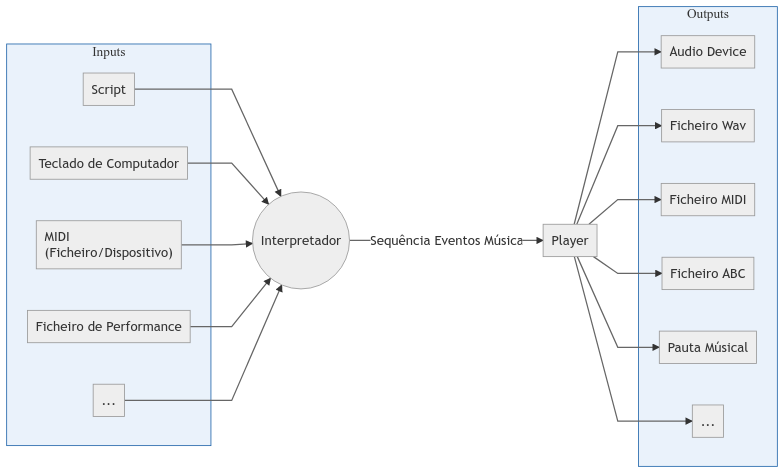
\includegraphics[width=0.87\textwidth]{img/diagram_architecture.png}
\end{center}
\caption{Arquitectura Geral do Projeto}
\end{figure}

O interpretador receberá um \textit{script} obrigatório como input. Esse input poderá depois determinar quais os \textit{inputs} (opcionais) que irá usar, como o teclado do computador, ficheiros ou teclados \acrshort{midi}, ficheiros de performance (gravações de reproduções anteriores consistindo nos eventos em que as teclas foram premidas).

Os eventos gerados pelo \textit{script} e os restantes \textit{inputs} serão depois redirecionados para os diversos \textit{outputs}, que podem ser as colunas do dispositivo, ficheiros \acrshort{wav} ou \acrshort{midi}, ficheiros em formato PDF com a pauta músical, entre outros.

Toda a linguagem irá ser desenvolvida com extensibilidade em mente nos seguintes pontos:
\begin{description}
    \item[Inputs] Permitir a criação de novos \textit{inputs}, como estar à espera de mensagens por um \textit{socket} ou de outros processos do computador.
    \item[Eventos] A linguagem já disponibiliza uma variedade de eventos multimédia (como reproduzir notas, sons genéricos, ou mensagens para controlar dispositivos \acrshort{midi}). Mas o objetivo é que criar e emitir eventos customizados seja extremamente simples (e feito com uma só linha de código por evento, no mínimo). Obviamente, nem todos os eventos são suportados por todos os outputs (por exemplo, um ficheiro ABC não pode reproduzir um ficheiro \acrshort{wav}), mas neste caso os diversos \textit{outputs} irão simplesmente ignorar os eventos que não estejam preparados para lidar.
    \item[Outputs] Para além dos \textit{outputs} embutidos, permitir criar novos, tanto para outros formatos músicais, mas também para outros fins como controlar luzes, vídeo e imagens através da linguagem (em conjunto com os eventos personalizados) e permitir assim executar espectáculos multimédia completos a partir da linguagem.
    \item[Bibliotecas] Expôr funções, variáveis e objetos adicionais, bem como possivelmente acrescentar dinamicamente sintaxe à linguagem (através de macros).
\end{description}


    % TODO Float H position
\begin{figure}[h]
\begin{center}
    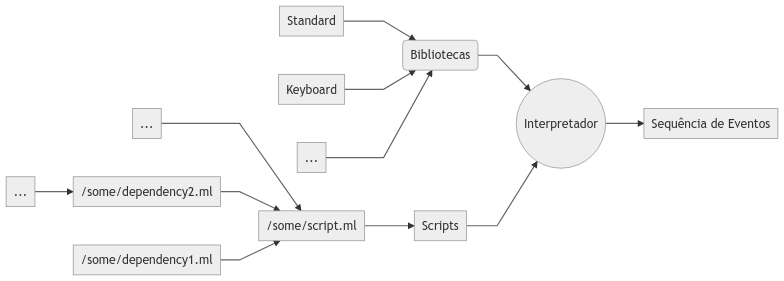
\includegraphics[width=0.95\textwidth]{img/diagram_virtualmachine.png}
\end{center}
\caption{Arquitectura do Interpretador}
\end{figure}
O facto de a linguagem ser desenvolvida em \textit{Python} significa que é extremamente prático extender a mesma devido a:
\begin{itemize}
    \item Ubiquidade da linguagem Python tanto para programadores experiêntes como para iniciantes;
    \item Não ser necessário compilar o código para o executar;
    \item Sintaxe e expressividade da linguagem (apesar de vezes isso incorrer num custo de performance);
    \item Existência de \textit{bindings} para bibliotecas desenvolvidas em C/C++ (como \textit{numpy}), optimizadas para inúmeras tarefas que necessitem de maior \textit{performance}/menor latência, que mesmo assim expôem uma interface agradável de usar em \textit{Python};
\end{itemize}
